\documentclass[a4paper]{article}
\usepackage{fullpage}
\usepackage{graphicx}
\usepackage[utf8]{inputenc}
\usepackage[portuguese]{babel}
\usepackage{indentfirst}
\usepackage{listings}

\lstset{language=Haskell}

\renewcommand{\baselinestretch}{1}

\author{João Reis\\
\texttt{A75372}
\and
Ricardo Pereira\\
\texttt{A74185}}
\date {Janeiro 2014}
\title{Relatório Laboratórios de Informática I}

 

\begin{document}

\maketitle
\section{Introdução}

Como projecto da disciplina Laboratórios Informática I, tivemos de programar em \textit{Haskell} um conjunto de funções que verificam e analisam diferentes aspectos da estrutura de um dado nível baseado no jogo \textit{Lightbot}, bem como maneiras para o completar.
O jogo, \textit{Lightbot}, com vários níveis, consiste num \textit{robot} que tem de percorrer um mapa diferentes com elevações e acender todas as lâmpadas, seguindo as instruções dadas inicialmente pelo jogador.

Um nível está divido em três diferentes partes: a primeira, que consiste no tabuleiro correspondente à área disponível para movimento do jogador, a segunda, que indica a coordenada onde o jogador começa, e por fim a terceira, que designa os movimentos para a solução correcta do mapa.

A primeira parte do projecto está dividida em três tarefas, cada qual com um diferente objectivo. A tarefa A, que consoante os níveis elaborados, tem de indicar se estes estão correctos (se este for o caso), ou então assinalar a linha que contem um erro. Na tarefa B, o programa têm de determinar a posição do jogador após a execução do primeiro comando presente nos movimentos que indicam a solução. Caso não esteja em conformidade com o mapa, por exemplo, saltar quando há uma lâmpada, deverá dar erro. Por fim, a tarefa C, lê os comandos presentes nos movimentos que indicam a solução, executa-os, verifica se acende todas as luzes, e se tal verificar-se, indica as coordenadas onde estão as lâmpadas e o numero de movimentos efectuados.

Por outro lado, a tarefa D, pertencente à segunda parte do mesmo projecto, consistiu em construir um programa que, dado um tabuleiro e as coordenadas iniciais devolve uma série de comandos para acender todas as lâmpadas. Finalmente, como pedido na Tarefa E, construiu-se uma animação 3D a partir de um dado nível.

\subsubsection{O jogo \textit{Lightbot}}
No jogo online, o robot percorre um tabuleiro até acender todas as luzes, seguindo comandos previamente dados pelo jogador.
O robot pode efectuar os seguintes comandos: 
\begin{itemize}
\item Ligar a lâmpada (L)
\item Avançar (A)
\item Virar para Esquerda (E)
\item Virar para a Direira (D)
\item Saltar (S)
\end{itemize}

O tabuleiro é diferente de nível para nível, podendo ter diferentes elevações. Para ser completado todas as luzes existentes no mapa terão de ser acendidas.


\subsubsection{Programação inicial: Haskell}
Como indica o título, Haskell é uma linguagem de programação puramente funcional. É a linguagem que é inicialmente leccionada no curso e portanto será a mesma utilizada no projecto.

\subsubsection{x3dom}
O x3dom é uma tecnologia utilizada para a renderização de objectos 3D em navegadores web.

\subsubsection{Mooshak e SVN}
A plataforma mooshak permitiu-nos avaliar a funcionalidade do nosso código segundo parâmetros definidos pelo pessoal docente da Unidade Curricular. Consoante a validade do código, maior a pontuação.

O subversion, conhecido como svn, permitiu-nos armazenar o nosso código, testes, relatório e a documentação, para maior facilidade de acesso dos membros do grupo assim como dos docentes.

\subsubsection{Documentação: \textit{haddock}}
O Haddock permitiu-nos documentar o nosso código de modo a formar um documento HTML com a explicação das funções do nosso programa.

\begin{figure}[!ht]
\centering
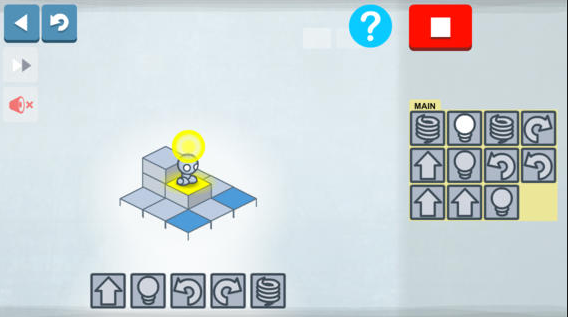
\includegraphics[width=0.6\textwidth]{lightbot.png}
\caption{\label{fig:figura 1} O Jogo: Lightbot.}
\end{figure}


\break
 

\section{Tarefas}
\subsection{Tarefa A}
A tarefa A tem como função analisar um tabuleiro constituído por linhas de texto que indicam três diferentes partes:

\begin{itemize}
\item \textbf{Mapa:} esta componente é constituída pelo espaço jogável, que indica as diferentes elevações do mapa assim como as coordenadas onde o robot tem que acender as lâmpadas.

\item \textbf{Coordenada Inicial}: Este espaço indica o local onde o robot está inicialmente, isto é, as coordenadas onde se encontra antes da execução comandos dados para movimento.

\item \textbf{Comandos}: Finalmente neste local encontra-se os comandos para os diferentes comportamentos do robot.

\end{itemize}

Se qualquer um destes aspectos for desrespeitado, o programa indicará onde se encontra a linha do erro, caso contrário, obtemos o resultado "OK".

\subsubsection{Função Principal}
Na Tarefa A, a função principal verifica se o nível cumpre todos os requisitos para estar de acordo com a estrutura correcta, passo-a-passo com recurso a funções auxiliares. Se tal se verificar, devolve uma string "OK", se não, devolve o numero da linha onde se encontra um erro.

\begin{lstlisting}[frame=single]
tarefa :: Nivel -> Resultado
\end{lstlisting}

Numa primeira parte verifica se esta têm o comprimento mínimo (3) para ser válida

\begin{lstlisting}[frame=single]
if limite l == False
then "1"
\end{lstlisting}

De seguida confere se as coordenadas estão conforme a estrutura padrão (coordenada X, coordenada Y e orientação), e posteriormente verifica se algumas das coordenadas, X ou Y, não têm maior comprimento ou altura do que o tabuleiro. Se algum dos anteriores aspectos não for cumprido, a função dá a linha onde as coordenadas de encontram.:

\begin{lstlisting}[frame=single]
else if coordenadas (head (doisUlt l)) == False 
|| coordenadasY l (yponto l) == False
|| coordenadasX l (xponto l) == False 
then show (length (init l))
\end{lstlisting}

Logo após, a função verifica se o mapa é todo ele constituído por letras e se tal se confirmar, averigua se todas as linhas têm o mesmo mesmo comprimento e da mesma maneira. Analogicamente, se algum destes aspectos não se confirmar a função devolve a linha onde se encontra o erro.
\begin{lstlisting}[frame=single]
else if length (mapa l) >= erro1 (mapa l) 
then show (erro1 (mapa l))
else if length (mapa l) >= erro2 (comp (mapa l)) (mapa l) 
then show (erro2 (comp (mapa l)) (mapa l))
\end{lstlisting}
Por fim, se anteriormente tudo estiver correcto, verifica se alguma linha é nula, e se tal não se verificar, devolve "OK"

\begin{lstlisting}[frame=single]
else if nulas l 
then show (erroN l)
else "OK"
\end{lstlisting}

A função \verb|erro1| indica a linha do tabuleiro que tiver um erro se este tiver caracteres que não sejam letras. Se tal não se verificar dará um numero maior que o numero de linhas que o do tabuleiro, e a função principal toma isto como correcto.

A função \verb|erro 2| indica a linha do tabuleiro que não tenha o mesmo comprimento que as restantes. Caso tal não se verifique, dará um numero maior que o numero de linhas que o do tabuleiro, e a função principal toma isto como correcto

\subsubsection{Testes}

Para averiguar a qualidade e funcionamento do código elaborado, recorremos à experimentação por testes. Desta maneira, criava-se um ficheiro .in para o programa ler, e um .out, que deverá ser o output vindo do programa.

Como exemplo, temos o ficheiro \verb|tA15.in|, que contêm o seguinte:
\begin{verbatim}
aacaD
aaBaa
bbCaa
1 0 S
SEMSLEAADSAL
\end{verbatim}

Se efectuarmos o comando \verb|testa|, obtemos o resultado, que deverá corresponder ao .out
\begin{verbatim}
>testa "tA15.in"
5
\end{verbatim}

Analogamente, para um teste com estrutura correcta, como \verb|tA01.in|:

\begin{verbatim}
aacdD
aaBaa
bbCaa
0 1 S
SEASLEAADSAL

>testa "tA01.in"
"OK"
\end{verbatim}
\break
\subsection{Tarefa B}

Nesta tarefa pretende-se elaborar um programa que determine a posição do robot após a execução do primeiro comando fornecido. Deverá seguir os seguintes aspectos:

\begin {itemize}
\item Os dados de entrada deverão estar em conformidade comidade com a Tarefa A;

\item Caso o comando seja aplicável à posição a que o robot se encontra, deverá ser apresentado as coordenadas correspondente à sua nova posição, bem como para onde está orientado.

\item Se tal não se verificar, como por exemplo, saltar quando há uma lâmpada, deverá retornar uma mensagem com "ERRO"

\end{itemize}
\subsubsection{Função Principal}
A função principal da Tarefa, recorrendo a várias funções auxiliares, analisa o primeiro comando para ver se é aplicável à posição onde está. Ou seja, testa todos os possíveis movimentos, e caso nenhum seja aplicável, devolve erro.

\begin{lstlisting}[frame=single]
tarefa :: Nivel -> Resultado
\end{lstlisting}
Inicialmente, a função verifica se o nível é nulo. Se tal se verificar, imprime "ERRO".
\begin{lstlisting}[frame=single]
tarefa l = if null l 
then "ERRO"
\end{lstlisting}
De seguida, verifica se o primeiro comando corresponde a uma rotação do robot, ou seja, direita (D) ou esquerda (E), e se tal for aplicável, recorrendo à função \verb|rotacao3|, a mesma devolve as coordenadas bem como a sua nova orientação.
\begin{lstlisting}[frame=single]
else if rotacao1 l 
then rotacao3 l (head(last l))
\end{lstlisting}
Posteriormente, verifica se o primeiro comando se trata de avançar (A). Caso se verifique, com recurso à função \verb|avancar4|, a mesma função verifica se é aplicável, e se assim o for devolve as novas coordenadas de onde se encontra o robot.
\begin{lstlisting}[frame=single]
else if avancarA l
then avancar4 l (last (last (init l)))
\end{lstlisting}
Consecutivamente, verifica se o primeiro comando corresponde ao salto (S), e se tal se confirmar, recorrendo à função \verb|avancar5|, esta devolve-nos a nova posição do robot se tal for aplicavel.
\begin{lstlisting}[frame=single]
else if avancarS l 
then avancar5 l (last (last (init l)))
\end{lstlisting}
Finalmente, a função verifica se o ultimo comando trata-se de uma lâmpada (L), e se for aplicável, a função \verb|lampada1| devolve as coordenadas iniciais.
\begin{lstlisting}[frame=single]
else if lampada l
then lampada1 l 
\end{lstlisting}
Se nenhum dos comandos anteriores (E,D,A,S ou L) é reconhecido, a função devolve "ERRO".
\begin{lstlisting}[frame=single]
else "ERRO"

\end{lstlisting}

\subsubsection{Testes}

Assim como na tarefa A, recorremos à experimentação para avaliar o funcionamento do código. Desta maneira, recorrendo novamente a ficheiros .in (para a leitura do programa) e ficheiros .out (correspondentes ao output vindo do programa.

Como exemplo, temos o ficheiro \verb|tB01.in|:
\begin{verbatim}
aacdD
Aacaa
bbCaa
3 1 S
EEASLEAADSAL
\end{verbatim}

Se efectuarmos o comando \verb|testa|, obtemos o resultado, que deverá corresponder ao .out
\begin{verbatim}
>testa "tB15.in"
3 1 E
\end{verbatim}


Analogamente, para um teste com suposto resultado incorrecto (\verb|tB23.in|):

\begin{verbatim}
aacdd
aacaa
bbCaa
4 2 E
AEASLEAADSAL
>testa "tB23.in"
ERRO
\end{verbatim}

\break
\subsection{Tarefa C}

Como ultimo programa da primeira parte a elaborar, nesta Tarefa têm-se de elaborar um conjunto de funções que façam o robot executar a sequência de comandos até acender todas as lâmpadas. Deverá seguir os seguintes aspectos:

\begin{itemize}
\item Os dados de entrada deverão estar em conformidade comidade com a Tarefa A;

\item Os comandos são executados em sequência, e os que não aplicaveis deverão deixar o estado do robot inalterado;

\item Assim que um comando L for executado correctamente deverá indicar as coordenadas a que se encontra

\item Assim que todas as lâmpadas estejam acesas, o programa indica "FIM" com o numero de comandos executados.

\item Se todas as lâmpadas não forem acesas, deverá aparecer "INCOMPLETO"
\end{itemize}

\subsubsection{Função Principal}
Na Tarefa C, a função principal recebe um nível, lê a sequencia de comandos e indica as coordenadas das luzes que se acenderam. Caso alguma não acenda, a função retorna as coordenadas das acesas assim como "INCOMPLETO".

Será importante referir que usou-se a tarefa B como suporte para a realização desta mesma tarefa.


\begin{lstlisting}[frame=single]
tarefa :: [String] -> String
\end{lstlisting}

Primordialmente, verifica se o nível é nulo:
\begin{lstlisting}[frame=single]
tarefa l = if null l 
then "INCOMPLETO"
\end{lstlisting}

De seguida compara o comprimento de duas listas: uma com as lâmpadas do jogo, e outra com o
numero de lâmpadas ligadas, dada pela função \verb|ligacao3|.
A função \verb|ligacao3| basicamente analisa a sequência do jogo, dado pela função sequenceF, e verifica as lâmpadas que ficaram ligadas. Caso o número seja igual, significa que o nível foi concluído com sucesso, e devolve como output as coordenadas das lâmpadas onde o comando L foi aplicável, e FIM seguido do numero de comandos bem aplicados.
\begin{lstlisting}[frame=single]
else if length (lines (result (ligacao3 (sequenceF l) 
(auxiliar4 (reverse (mapa l)) 0 0) []))) == 
length (auxiliar4 (reverse (mapa l)) 0 0)
then unlines (verifica2 (sequenceF l)) ++ "FIM " ++ 
(show (verificar1 (sequenceF l) (ligacao4 (sequenceF l) 
(auxiliar4 (reverse (mapa l)) 0 0) [] )))
\end{lstlisting}

Finalmente, se isso não se verificar, devolve as coordenadas das lâmpadas acesas, seguido de "INCOMPLETO"
\begin{lstlisting}[frame=single] 
else unlines (verifica2 (sequenceF l)) ++ "INCOMPLETO" 
\end{lstlisting}

\subsubsection{Testes}
Tal como nas tarefas anteriores, recorremos novamente à experimentação para verificar a validade do programa, usando ficheiros .in, para leitura do programa, e .out, correspondente à resposta à resposta do mesmo.

Como exemplo, temos o ficheiro \verb|tC01.in|, que contêm o seguinte:
\begin{verbatim}
aacdD
aacaa
bbCaa
0 1 S
SEASLEAADSAL
\end{verbatim}

Se efectuarmos o comando \verb|testa|, obtemos o resultado, que deverá corresponder ao .out
\begin{verbatim}
>testa "tC01.in"
2 0
4 2
FIM 12
\end{verbatim}

Analogamente, para o teste com suposto resultado incorrecto (\verb|tC08.in|):
\begin{verbatim}
aD
bb
0 1 S
SESESL

>testa "tC08.in"
INCOMPLETO
\end{verbatim}

\break
\subsection{Tarefa D}
Como quarta tarefa de projecto a elaborar, terá de ser criado um programa que dado um tabuleiro e os a coordenadas iniciais, faça o robot percorrer o mapa de modo a acender todas as lâmpadas presentes.
Tem de respeitar os seguintes aspectos:
\begin{itemize}
\item Lê um ficheiro de entrada, que contêm o tabuleiro assim como as coordenadas iniciais.
\item Imprime os comandos necessários para acender todas as luzes do tabuleiro.

\subsubsection{Desenvolvimento}

Na tarefa D, a função principal (\verb|tarefa|) irá apenas fornecer dados à função \verb|tarefa2|, que funciona como motor de todo o programa. 
A função \verb|tarefa2| recebe um nível, uma posição e uma lista Int, das coordenadas das lâmpadas. Caso não seja possível deslocar-se, aplica as funções pela ordem inversa, ou seja, \verb|igualX|, e só depois \verb|igualY|, deslocando-se na mesma em L. Caso não seja possivel a aplicação da função \verb|igualY|, aplica-se as funções pela ordem inversa, e vice-versa para a função \verb|igualX|. No entanto, caso nenhuma destas formas sejam possíveis, a tarefa muda a ordem da lâmpada a acender, caso a lista das coordenadas seja igual ou superior a dois. Finalmente, como ultimo caso, temos a função parede, isto se aparecer obstáculos.

\subsubsection{Testes}

Para testar a validade de funcionamento do código desta Tarefa, verificamos os outputs dados pelo programa criando um nivel com os comandos dados e testa-los na Tarefa C, pois esta iindica se o nível é completo ou não.

Como exemplo, o seguinte nível:
\begin{verbatim}
aacdD
aacaa
bbCaa
0 1 S
\end{verbatim}

Pode ter o output:
\begin{verbatim}
SEASLEAADSAL
\end{verbatim}

\end{itemize}
\break
\subsection{Tarefa E}
Por fim, como ultima tarefa de todo o projecto, terá de se elaborar um programa em Haskell que forneça um código x3dom para a animação 3D de um nível.
Terá de seguir os seguintes aspectos:

\begin{enumerate}
\item Lê o ficheiro de entrada que dá um tabuleiro, as coordenadas (que indicam a posição inicial) e os comandos para acender as luzes.

\item Dado o ficheiro de entrada, o programa criará um ficheiro HTML com o elemento x3dom que representa a animação 3D de um dado nivel.

\item Na animação, o robot percorrerá o mapa de modo a acender as luzes.

Para melhor estética, a página que contem o elemento x3dom foi personalizada com auxilio a HTML e CSS.
\end{enumerate}

\subsubsection{Desenvolvimento}

Inicialmente, na tarefa E começamos por personalizar a página que iria ser criada pelo programa. Com auxilo a HTML e CSS, personalizamos uma página para melhor estética.

De seguindo adoptamos o estilo e adaptamos ao resultado vindo do programa realizado em Haskell.

A função \verb|tarefa| é a função que gera o código HTML consoante o nivel aberto. Esta já tem parte código HTML, que é igual para todos, e corresponde à personalização que fizemos anteriormente. Portanto, pode-se verificar que todo o código será semelhante, divergindo apenas nos cubos que representam o mapa, assim como a rota que o robot adopta: para tal, as funções \verb|formaLamp| (forma um cubo que corresponde à lâmpada), \verb|formaTab2| (forma o restantes cubos do tabuleiro), \verb|formaRobot| (forma o robot, com as coordenadas e orientação inicial) e \verb|formaRota| (forma a rota do robot, bem como a variação do tempo) dão o código para a parte que sofre variação.

\break

\section{Conclusão}

Como forma de introdução ao mundo da programação, a Unidade Curricular Laboratórios de Informática permitiu-nos perceber as aplicações da linguagem funcional Haskell.


Após muito tempo despendido nas Tarefas, estas levaram-nos a concluir que quando programando, a experimentação e a paciência são valores chave para seja efectuada correctamente.


Foi-nos claro que testar seria uma parte vital do projecto assim que o começamos, dado que para verificarmos a validade do nosso código a solução passaria por experimentar o conjunto de funções que elaboramos a diferentes situações. Ao testar, viriam erros e respostas indesejadas, estes que só com paciência e insistência teríamos a capacidade de os localizar e emendar.


Em suma, foi um projecto que nos acomodou à programação, e com os problemas que viriam da sua experimentação, a calma nos momentos mais difíceis são aspectos chave os solucionar.
\end{document}